\section{Phase 4 - Clustering and Association}

\subsection{K-means++}

K-means is a classic algorithm for clustering, a method of vector quantization that groups similar data points into clusters. It's a type of unsupervised learning algorithm that's used when data is unlabeled. However, a drawback of K-means is that it could lead to bad arbitrary clusters. K-means++ is a method of choosing initial values for K-means. Instead of choosing randomly, K-means++ spreads them out evenly.

This part of the project demonstrates the optimization of k using elbow method and silhouette analysis.

For each candidate k, run a \texttt{sklearn.cluster.\_kmeans.KMeans} model with the parameter \texttt{init} set to "k-means++". Then, calculate SSE based on euclidean distance, and silhouette score using \\ \texttt{sklearn.metrics.cluster.\_unsupervise.silhouette\_score}.

Figure~\ref{fig:kmeans-elbow} shows the procedure of elbow method optimization on k-means. The knee of th eplot is observed at $k = 6$, while in the silhouette analysis shown in figure~\ref{fig:kmeans-sil}, the silhouette score of 7 is greater than 6. Based on both elbow method and silhouette score, the number of clusters is set to 7 for clustering.

\begin{figure}
    \centering
    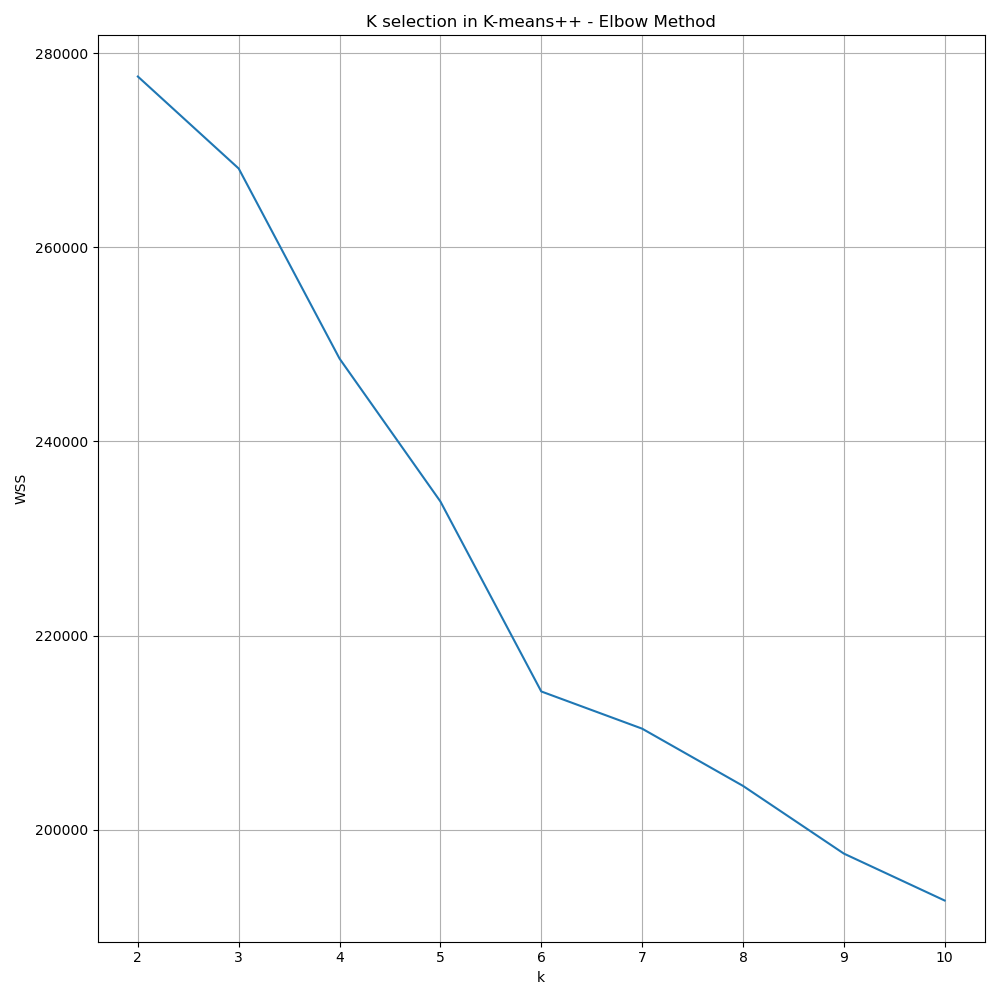
\includegraphics[width=1\linewidth]{docs//assets/kmeans_elbow_method.png}
    \caption{Elbow Method to Optimize K-means}
    \label{fig:kmeans-elbow}
\end{figure}

\begin{figure}
    \centering
    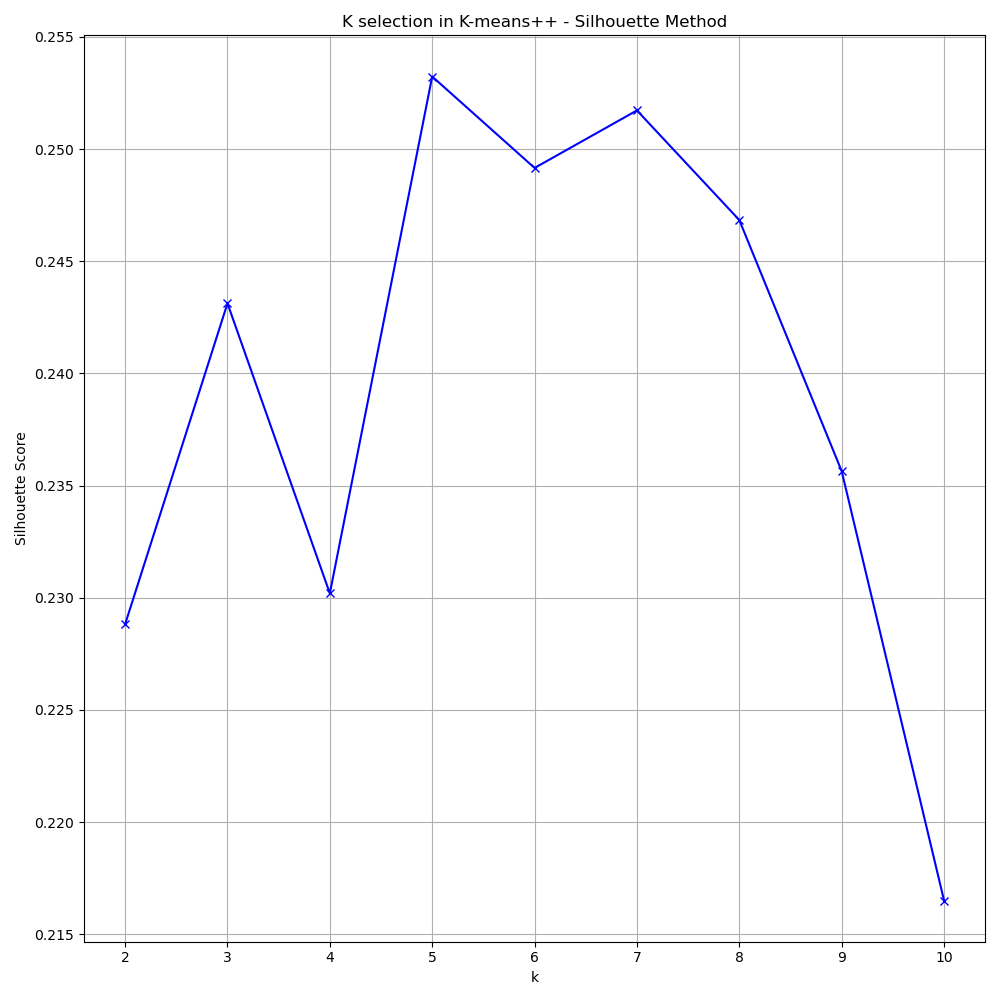
\includegraphics[width=1\linewidth]{docs//assets/kmeans_silhouette_method.png}
    \caption{Silhouette Analysis to Optimize K-means}
    \label{fig:kmeans-sil}
\end{figure}

In order to visualize the dataset on a 2D plot, PCA is used to transform the multi feature dataset into a 2-components matrix, where can interpreted as points to be placed on a 2D plot. Figure~\ref{fig:pca-kmeans} shows that the clusters are spread and not overlapping much, suggesting a reasonable choice of k.

\begin{figure}
    \centering
    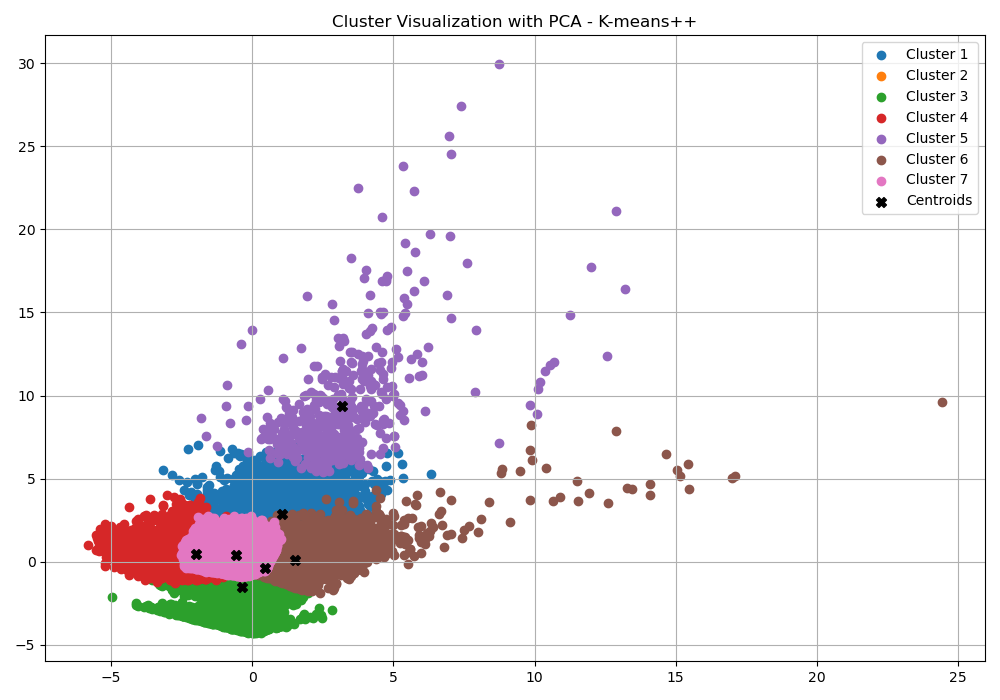
\includegraphics[width=1\linewidth]{docs//assets/Cluster Visualization with PCA - K-means++.png}
    \caption{Cluster Visualization with PCA - K-means++}
    \label{fig:pca-kmeans}
\end{figure}

\subsection{DBSCAN}

Figure~\ref{fig:pca-dbscan} shows the distribution of clusters using DBSCAN algorithm. Initially, the algorithm emits over a hundred clusters. In order to display the maximum information, the figure only chose the top 10 clusters with the most observations. It can be observed that the shape of cluster 6 in figure~\ref{fig:pca-dbscan} is similar to cluster 3 in figure~\ref{fig:pca-kmeans}, suggesting a common cluster observed in the same dataset, verifying the result of cluster distribution.

\begin{figure}
    \centering
    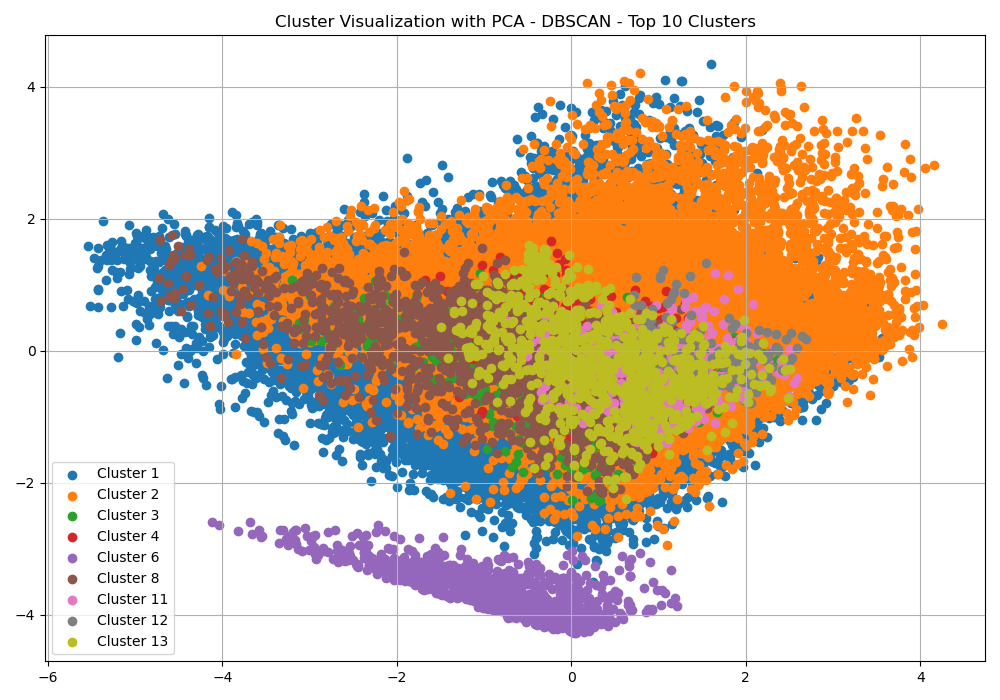
\includegraphics[width=1\linewidth]{docs//assets/Cluster Visualization with PCA - DBSCAN - Top 10 Clusters.png}
    \caption{Cluster Visulization with PCA - DBSCAN}
    \label{fig:pca-dbscan}
\end{figure}


\subsection{Association Rule with Apriori Algorithm}




To begin with, the dataset is further cleaned for the association rule analysis. Table~\ref{tab:ar-dataset} shows the cleaned dataset for association rule mining.

\begin{table}
    \centering
    \scriptsize
    \begin{tabular}{rrrrrrr}
        \toprule
         cat\_Prod &  cat\_Social &  isInAppPur &  rating\_High &  appAge\_Old &  lastUp\_Old &  size\_Large \\
        \midrule
         0 &   0 &   0 &    0 &    1 &    0 &    0 \\
         0 &   0 &   1 &    0 &    1 &    1 &    0 \\
         0 &   0 &   1 &    0 &    1 &    1 &    0 \\
         0 &   0 &   0 &    1 &    1 &    0 &    0 \\
         0 &   0 &   1 &    0 &    1 &    1 &    0 \\
        \bottomrul
    \end{tabular}
    \caption{Dataset for Association Rule}
    \label{tab:ar-dataset}
\end{table}

After dataset is well prepared, run Apriori algorithm,\\ \texttt{mlxtend.frequent\_patterns.apriori} is utilized for this purpose. The parameter chose for the initialization is the minimum support. Support is the percentage of frequency of item set vs all observations. After all item set that satisfy the min\_support is taken into account, the return value of apriori algorithm is all the items set calculated.

Table~\ref{tab:apriori} shows the support and the item set of all the qualifying item sets.




\begin{table}
\scriptsize
    \centering
    \begin{tabular}{cr}
    \toprule
        Support & Itemsets \\
        \midrule
        0.025 & {cat\_Prod} \\
        0.019 & {cat\_Social} \\
        0.281 & {isInAppPur} \\
        0.193 & {rating\_High} \\
        0.922 & {appAge\_Old} \\
        0.410 & {lastUp\_Old} \\
        0.025 & {sizeInMB\_Large} \\
        0.023 & {appAge\_Old, cat\_Prod} \\
        0.016 & {appAge\_Old, cat\_Social} \\
        0.062 & {isInAppPur, rating\_High} \\
        0.252 & {appAge\_Old, isInAppPur} \\
        0.088 & {isInAppPur, lastUp\_Old} \\
        0.015 & {isInAppPur, sizeInMB\_Large} \\
        0.175 & {appAge\_Old, rating\_High} \\
        0.061 & {rating\_High, lastUp\_Old} \\
        0.410 & {appAge\_Old, lastUp\_Old} \\
        0.020 & {appAge\_Old, sizeInMB\_Large} \\
        0.054 & {appAge\_Old, isInAppPur, rating\_High} \\
        0.013 & {isInAppPur, rating\_High, lastUp\_Old} \\
        0.088 & {appAge\_Old, isInAppPur, lastUp\_Old} \\
        0.011 & {appAge\_Old, isInAppPur, sizeInMB\_Large} \\
        0.061 & {appAge\_Old, rating\_High, lastUp\_Old} \\
        0.013 & {appAge\_Old, isInAppPur, rating\_High, lastUp\_Old} \\
\end{tabular}
    \caption{Result of Apriori}
    \label{tab:apriori}
\end{table}

Next, generate association rules with lift as the metric. Lift displays the ratio of confidence for the rule to the prior probability of having the rule prediction. The minimum threshold chose for lift is \textbf{0.6}

\begin{table}
    \centering
    \scriptsize
        \begin{tabular}{rcccc}
        \toprule
        Antecedents & Consequents & Support & Confidence & Lift \\
        \midrule
        {isInAppPur, rating\_High, lastUp\_Old} & {appAge\_Old} & 0.013 & 1.000 & 1.085 \\
        {rating\_High, lastUp\_Old} & {appAge\_Old} & 0.061 & 1.000 & 1.085 \\
        {isInAppPur, lastUp\_Old} & {appAge\_Old} & 0.088 & 1.000 & 1.085 \\
        {lastUp\_Old} & {appAge\_Old} & 0.410 & 1.000 & 1.085 \\
        {cat\_Prod} & {appAge\_Old} & 0.023 & 0.937 & 1.017 \\
        {rating\_High} & {appAge\_Old} & 0.175 & 0.910 & 0.987 \\
        {isInAppPur} & {appAge\_Old} & 0.252 & 0.897 & 0.973 \\
        {isInAppPur, rating\_High} & {appAge\_Old} & 0.054 & 0.871 & 0.944 \\
        {cat\_Social} & {appAge\_Old} & 0.016 & 0.865 & 0.939 \\
        {size\_Large} & {appAge\_Old} & 0.020 & 0.773 & 0.838 \\
        {isInAppPur, size\_Large} & {appAge\_Old} & 0.011 & 0.729 & 0.791 \\
        {size\_Large} & {isInAppPur} & 0.015 & 0.610 & 2.168 \\
        {appAge\_Old, size\_Large} & {isInAppPur} & 0.011 & 0.575 & 2.046 \\
        \end{tabular}
    \caption{Association Rule}
    \label{tab:ar}
\end{table}

Table~\ref{tab:ar} displays the association rule of the dataset. The association rules are sorted by confidence, which is a percentage value that shows how frequently the rule head occurs among all the groups containing the rule body. The feature \texttt{appAge\_Old} is a variaty of high-confidence rules' consequents, meaning that the longevity of the app can be resulted from many conditions, such as having In-App-Purchases and a high rating.

Interestingly, the \textbf{\texttt{size\_Large} $\rightarrow$ \texttt{isInAppPur}} rule has 61\% of confidence, suggesting that when the size of an app gets larger, it is likely to have In-App-purchases.